\documentclass[cn,11pt,color=blue]{elegantbook}


\title{计网面试集合}
\subtitle{无题}
\author{宋鑫旺}
\institute{CoderHub}
\date{\today}
\version{0.01}

\extrainfo{Victory won\rq t come to us unless we go to it. --- M. Moore}

\logo{logo.png}
\cover{cover.jpg}


\begin{document}
	

\maketitle
\tableofcontents

% \thispagestyle{empty}

\mainmatter
\hypersetup{pageanchor=true}

\chapter{综合问题}

% -------------- 问题1 ----------------
\begin{custom}{问题1}
从浏览器地址栏输入 url 到显示主页的过程?
\end{custom}

\begin{solution}
这道题,大概的过程比较简单,但是有很多点可以细挖:DNS解析、TCP三次握手、HTTP报文格式、TCP四次挥手等等。
\begin{enumerate}
\item DNS 解析:将域名解析成对应的 IP 地址。
\item TCP 连接:与服务器通过三次握手,建立 TCP 连接
\item 向服务器发送 HTTP 请求
\item 服务器处理请求,返回 HTTP 响应
\item 浏览器解析并渲染页面
\item 断开连接:TCP 四次挥手,连接结束
\end{enumerate}

我们以输入 www.baidu.com 为例,过程如下图\ref{fig1_1} 所示:
\begin{figure}[htbp]
\centering
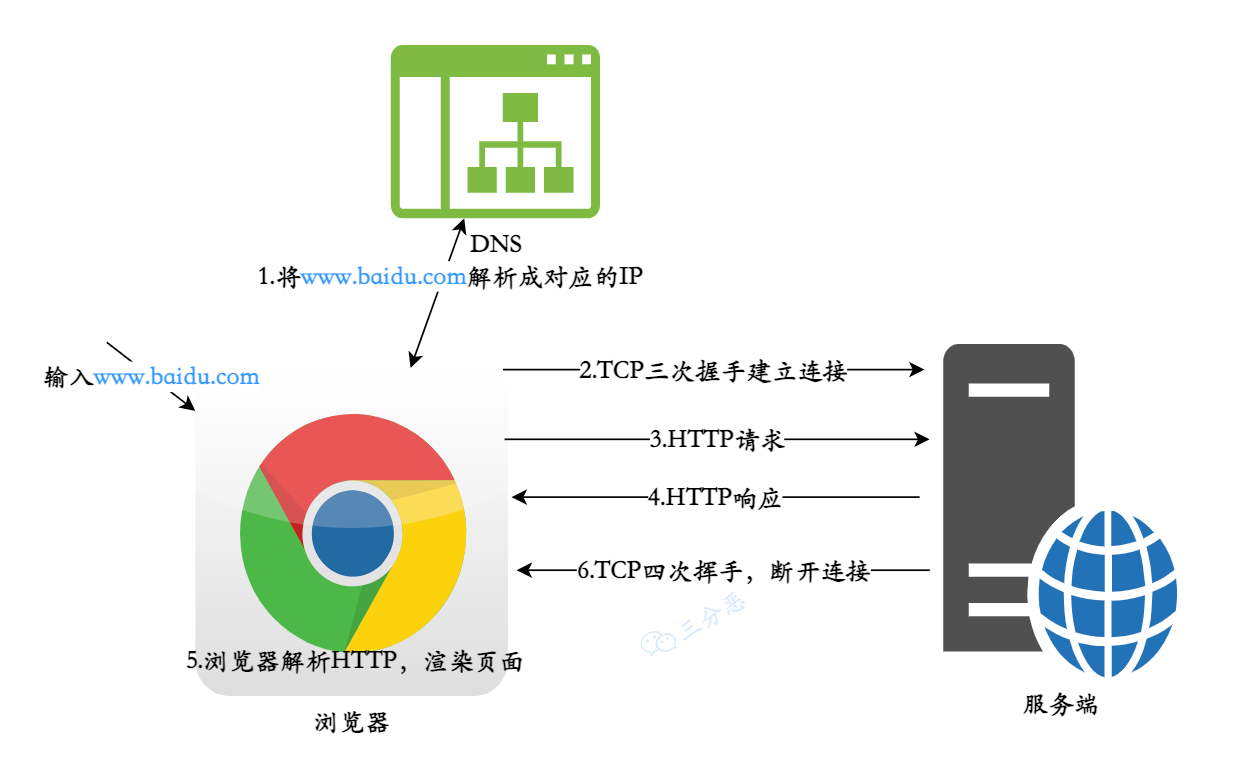
\includegraphics[width=0.95\textwidth]{./Chapter1/q1_1.png}
\caption{浏览器地址输入到显式主页的过程}
\label{fig1_1}
\end{figure}

各个过程使用到的协议如下图\ref{fig1_2} 所示:
\begin{figure}[htbp]
\centering
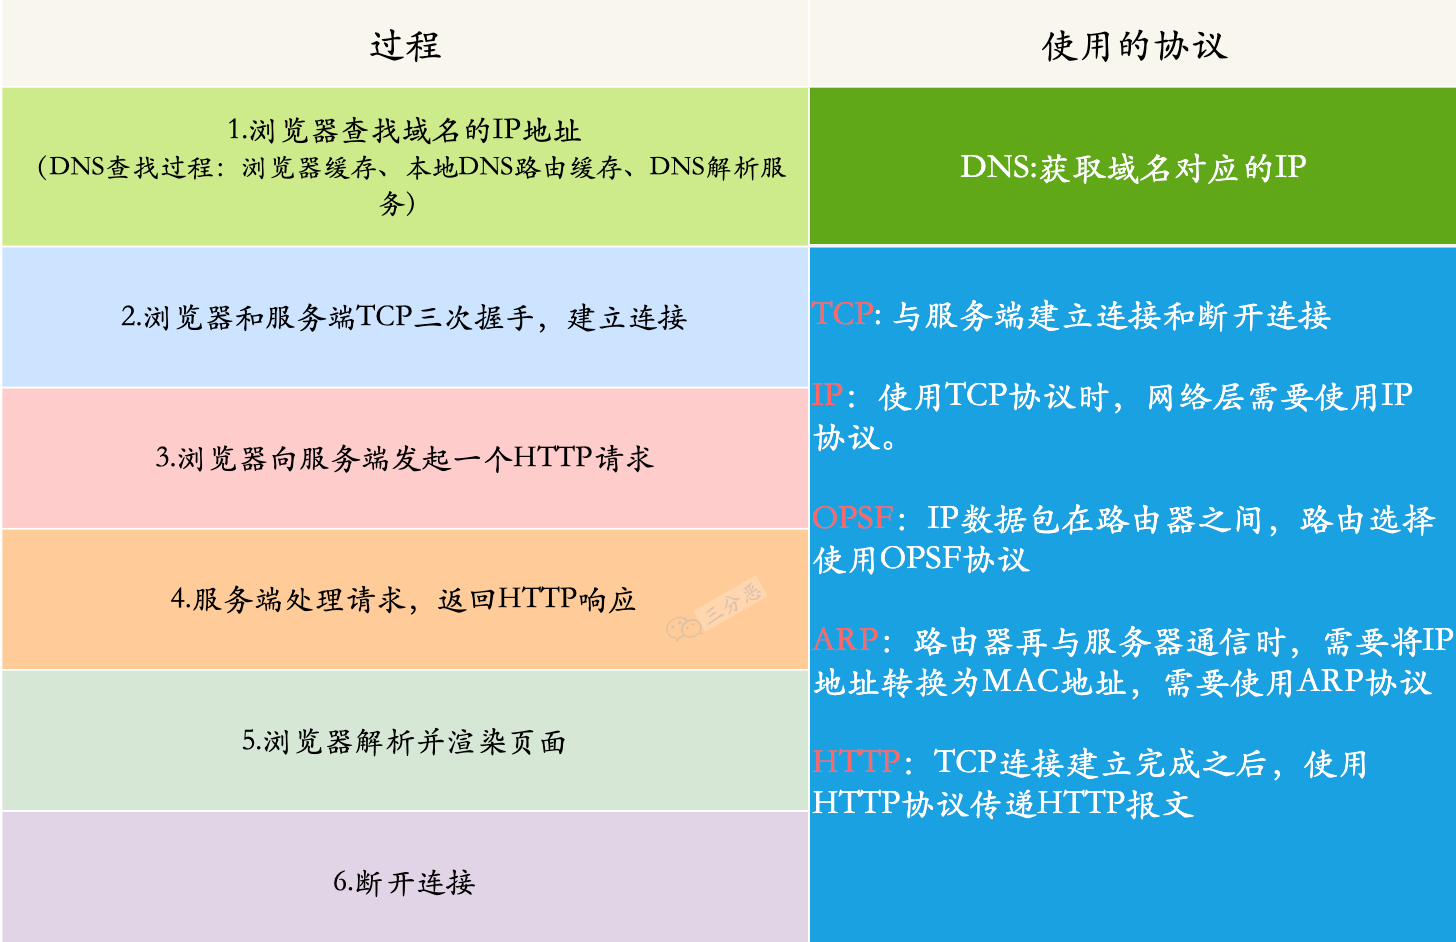
\includegraphics[width=0.95\textwidth]{./Chapter1/q1_2.png}
\caption{每个过程涉及到的协议}
\label{fig1_2}
\end{figure}
\end{solution}

% ----------------------- 问题2 ----------------------
\begin{custom}{问题2}
输入网址到渲染界面过程?
\end{custom}
\begin{solution}
发送http请求--->看本地缓存--->DNS解析出域名对应的IP地址--->TCP/IP五层协议--->可能会有代理(正向代理反向代理)--->TCP连接三次握手 / https认证,加密,解密--->找到端口号--->nignx反向代理将请求分发到具体服务器主机--->mvc框架下从views找到路由--->验证权限--->解析url参数--->看服务器中的缓存--->代码逻辑中获取数据并返回html模板--->服务端发送http响应--->浏览器渲染页面
\end{solution}

% ----------------------- 问题3 ---------------------
\begin{custom}{问题3}
正向代理和反向代理区别?
\end{custom}
\begin{solution}
首先代理是指:客户端主机借助代理服务器访问目标服务器。
\begin{itemize}
\item 客户端 -request-> 代理 -request-> 服务器
\item 客户端 <-response- 代理 <-response- 服务器
\end{itemize}

正向代理:客户端借助代理访问无法访问的服务器,客户端需要配置。

反向代理:服务端借助代理实现负载均衡,客户端无需配置,也不知道自己经过了代理。
\end{solution}

% ------------------ 问题4 ------------------------
\begin{custom}{问题4}
说一下你了解的端口及对应的服务
\end{custom}
\begin{solution}
常用的端口和作用如下图\ref{fig4_1} 所示:
\begin{figure}[htbp]
\centering
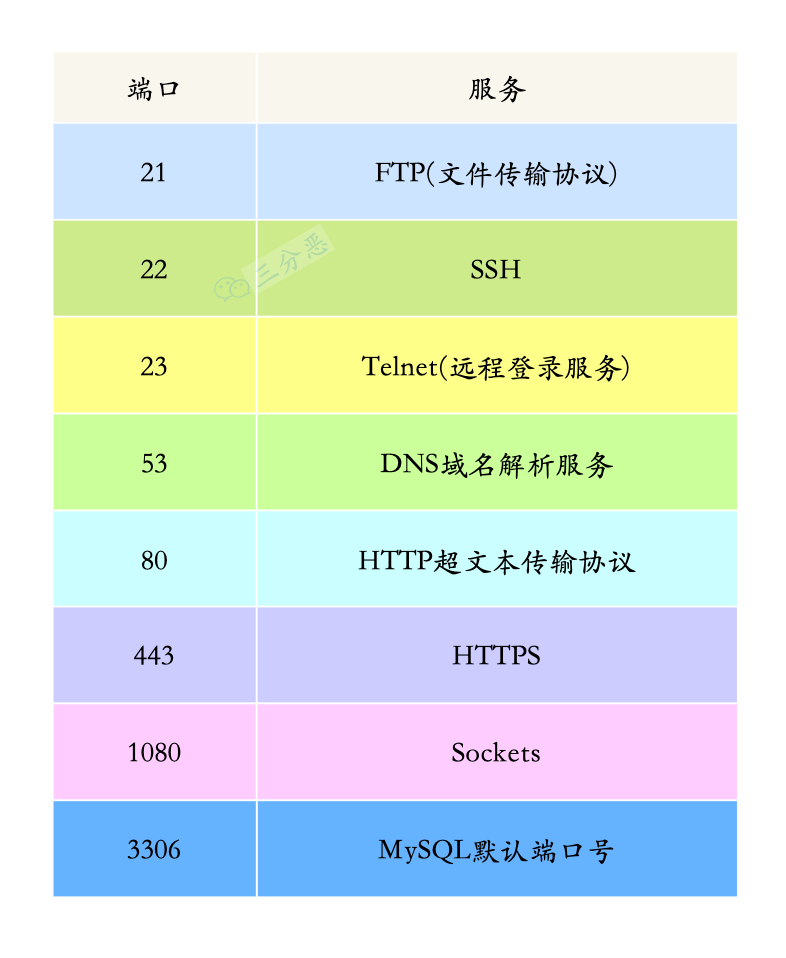
\includegraphics[width=0.95\textwidth]{./Chapter1/q4_1.png}
\caption{常见端口及对应服务}
\label{fig4_1}
\end{figure}

\end{solution}

% ---------------------- 问题5 ----------------
\begin{custom}{问题5}
介绍一下CDN?
\end{custom}
\begin{solution}
视频讲解链接:\href{https://www.zhihu.com/zvideo/1338850254489939968}{https://www.zhihu.com/zvideo/1338850254489939968},后续需要文字整理一下。
\end{solution}

% --- 问题6 ---
\begin{custom}{问题6}
cookie跨域
\end{custom}
\begin{solution}
目前还没有写答案,需要更新
\end{solution}



\end{document}
